\documentclass[a4paper]{article}

\usepackage[french]{babel}
\usepackage[utf8]{inputenc}
\usepackage{amsmath}
\usepackage{graphicx}
\usepackage{moreverb}
\usepackage{listings}
\usepackage[colorinlistoftodos]{todonotes}

\lstset{language=C++,
                basicstyle=\ttfamily\small,
                keywordstyle=\color{blue}\ttfamily,
                stringstyle=\color{red}\ttfamily,
                commentstyle=\color{gray}\ttfamily,
                morecomment=[l][\color{magenta}]{\#}
}

\title{Rapport d'implementation : High Resolution Sparse Voxel DAG}

\author{Etienne Ferrier et Nikolai Morin}

\date{}

\begin{document}
\maketitle

\begin{abstract}
Ce rapport decrit notre implementation partielle du papier \textit{High Resolution Sparse Voxel DAGs} [Kämpe, Sintorn, Assarsson, 2013].
\end{abstract}

\section{Objectif de la publication originale}
Ce papier décrit comment construire, stocker et manipuler des Sparse Voxel Directed Acyclic Graphs (DAG) afin de décrire une scène 3D de voxels. Les DAG sont une évolution des Sparse Voxel Octrees (SVO), qui permettent eux aussi de décrire une scène de voxels plus efficacement qu’une simple grille 3D.

Dans ce papier, les octrees et DAG sont utilisés en tant que descripteurs d’une scène 3D et non seulement en tant que structures d’accélération.

L’intérêt des DAG est qu’ils permettent d’encoder l’information d'une scène de voxels de façon plus compacte qu’un SVO tout en ayant une structure efficace vis-à-vis des algorithmes de lancer de rayon.


\section{Implementation}
L'implementation de l'algorithme de conversion a été réalisé en C++ en utilisant les libraries Glut/OpenGL. Afin de comprendre toutes les étapes du pipeline (voir Figure 1) du mesh au DAG, nous avons décidé de réaliser notre implémentation à partir du projet OpenGL de base du TD. Nous avons ajouté trois classes, décrites ci-dessous. \\

Les papiers sur les DAG ainsi que \textit{Efficient Sparse Voxel Octrees} [Laine, Karras, 2010] nous ont servi de référence. \\ 

Afin de comprendre toutes les étapes du pipeline (voir Figure 1) du mesh au DAG, nous avons décidé de réaliser notre implémentation à partir du projet OpenGL de base de la partie pratique du cours. Nous avons donc aussi implémenté notre propre conversion d’un maillage 3D vers un SVO grâce à une méthode de lancer de rayons.

\begin{figure}
\centering
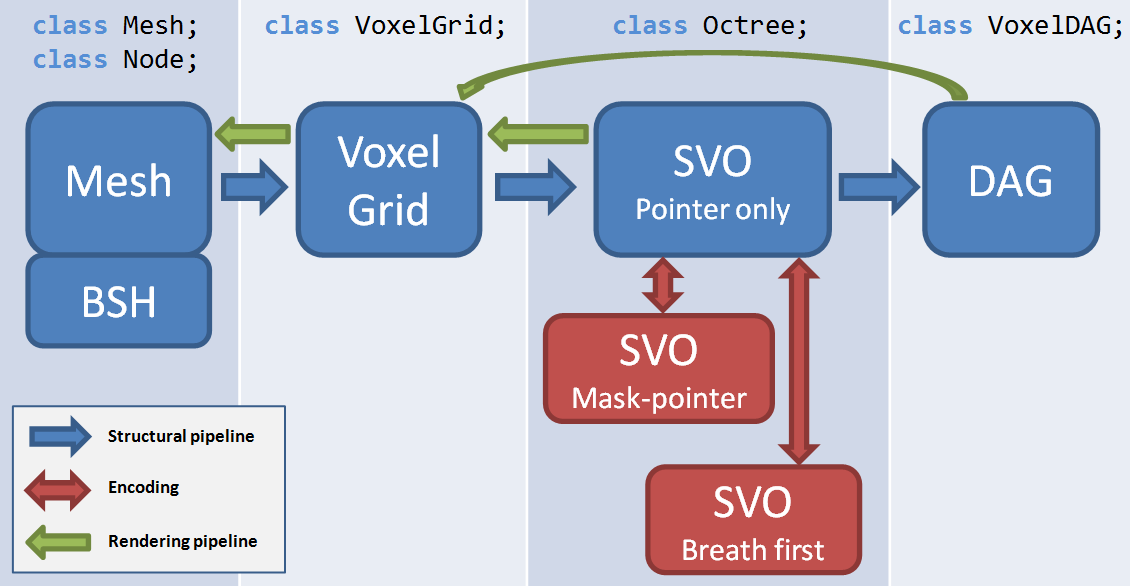
\includegraphics[width=1\textwidth]{ClassGraph.png}
\caption{\label{fig:triceratops}\textit{Pipeline of our implementation}}
\end{figure}


\subsection{Octree}
La classe Octree permet de construire un SVO à partir d'une VoxelGrid. Cette premiere structure de SVO est intuitive et son parcours (lancer de rayons) est efficace. Sa structure est récursive.

\begin{lstlisting}
 class Octree {
 	Octree* _children; // = NULL ou Octree[8]
 	bool _isEmpty;
 };
\end{lstlisting}

Chaque nœud qui n’est pas une feuille, i.e qui ne représente pas un voxel, contient 8 pointeurs vers ses nœuds fils. La location d'un voxel est définie par le chemin de la racine au nœud voxel. Cette classe permet de construire deux autres représentations, qui reposent sur les childmasks. \\ 

\subsubsection{Breadth first} % (fold)
\label{ssub:breadth_first}
Une représentation très compacte de SVO est la représentation \textit{breadth first}  dont le stockage est très réduit mais dont le parcours est inefficace. Pour chaque nœud intérieur, on peut calculer un masque de 8 bits décrivant l’occupation de ses fils. Les childmaks de tous les noeuds intérieurs sont enchainés dans l’ordre « largeur d’abord » dans un vecteur. La taille du vecteur en octets est donc égale au nombre de nœuds intérieurs. \\

La conversion se fait par la méthode suivante:
\begin{lstlisting}
void Octree::encodeBreadthFirst(
	std::vector<uint8_t>& storage);
\end{lstlisting}
% subsubsection breadth_first (end)


\subsubsection{Childmasks à indices} % (fold)

Nous avons aussi implémenté une représentation efficace \textit{mask-index} de SVO, similaire à celle de Laine et Karras. Les fils non vides d'un nœud sont stockés de manière consécutive et chaque childmask (jusqu'à l'avant-dernier niveau) est accompagné d'un entier correspondant à l'indice du premier fils non-vide. Cet encodage est plus compact que celui du SVO récursif et son parcours est efficace. La taille totale est celle de la représentation \textit{breadth-first} plus celle des indices. Souvent on juxtapose les deux nombres dans un entier de 32 bit, dont 24 pour l'index et 8 pour le childmask. \\

La conversion se fait par la méthode suivante dans notre implémentation :
\begin{lstlisting}
void Octree::encodeWithPointers(std::vector<uint8_t>& masks, 
	std::vector<int>& pointers);
\end{lstlisting}

Pour chaque nœud d'index i, son masque est stocké dans \texttt{masks[i]} et l’index de son premier fils non vide est stocké dans \texttt{pointers[i]}.



\subsection{VoxelDAG} % (fold)
La classe VoxelDAG calcule une structure efficace de DAG dont le stockage est réduit et dont le parcours est efficace. La représentation \textit{breadth first} est partionnée selon les niveaux de profondeur de l'octree, grâce à la fonction :
\begin{lstlisting}
std::vector<std::vector<std::vector<int>>> 
	VoxelDAG::buildFullSVO(Octree& oct);
\end{lstlisting}

Les vecteurs les plus intérieurs (de type \texttt{vector<int>}) décrivent chacun un nœud. Le premier élément est toujours le childmask, et les éléments suivants sont des indices vers des nœuds au niveau du dessous (les fils du noeud). Tous les nœuds d'un niveau sont stockés dans un vecteur et tous les niveaux de l'arbre forment donc la structure qui est rétourné. \\

Cette représentation convient à l'étape de fusion, pour chaque niveau, des nœuds qui ont le même childmask et les mêmes pointeurs. Comme \texttt{operator==} de \texttt{vector<int>} réalise cette comparaison, on peut utiliser les outils de la bibliothèque standard de C++. On procède du niveau des feuilles à celui de la racine de la manière suivante: \\

\begin{lstlisting}
// find all uniques
std::vector<std::vector<int>> uniques(dagTree[lvl]);
std::sort(uniques.begin(), uniques.end());
auto resizeIterator = 
	std::unique(uniques.begin(), uniques.end());
uniques.resize( std::distance(uniques.begin(),
	resizeIterator));

// merging
// find an (injective) mapping from the nodes
// in the original level to uniques
std::vector<int> mapping;
for (auto node : dagTree[lvl]) {
    auto newIt = std::lower_bound(uniques.begin(), 
    	uniques.end(), node);
    mapping.push_back(std::distance(uniques.begin(),
    	newIt));
}

// update the pointers in the level above to point
// to the same element in uniques
for (int prnt = dagTree[lvl-1].size() - 1; prnt >= 0; --prnt) {
    for (int i = dagTree[lvl-1][prnt].size() - 1; i > 0; --i) {
        dagTree[lvl-1][prnt][i] = 
        	mapping[dagTree[lvl-1][prnt][i]];
    }
}

// actually replace the level with its uniques
dagTree[lvl] = uniques;
\end{lstlisting}
Cette méthode réduit un arbre à un graphe orienté acyclique. Il serait possible d'optimiser, par enchaînement des nœuds et par un stockage qui juxtapose les childmasks et les indices, la taille finale du DAG.\\


Nous avons de plus ajouté une méthode :
\begin{lstlisting}
void VoxelDAG::toVoxelGrid(VoxelGrid& voxGrid);
\end{lstlisting}
qui sert à reconvertir le DAG en VoxelGrid, qui peut à son tour être facilement convertie en un maillage.

\subsection{Visualisation} % (fold)
\label{sub:visualisation}

Afin de visualiser la distribution des voxels à travers nos structures, nous avons implémenté des commandes clavier permettant :
\begin{itemize}
 \item (touche 'o') d'afficher successivement en orange les 8 sous octrees de la racine. 
 \item (touche 'd') d'afficher successivement en orange les feuilles du DAG afin de visualiser les blocs identiques de taille $2^3$ qui ont été fusionnés lors de la conversion du SVO.
 \item (touche 'c') de réinitialiser l'affichage.
\end{itemize}

% subsection visualisation (end)

\subsection{Résultats} % (fold)
\label{sub:r_sultats}
Nous avons pu comparer les résultats de ces différentes structures et observer l'utilité des DAG. Nous avons constaté qu'il faut souvent faire un choix entre stockage optimal et facilité de parcours.
% subsection r_sultats (end)

% \subsection{Extensions} % (fold)
% \label{sub:extensions}
% On s'est limité à une implémentation partielle. Des extensions possibles seraient:
% \begin{itemize}
%   \item Stockage plus efficace: toutes les données dans un seul vector
%   \item Rendu direct des SVO/DAG
%   \item Optimisation de la performance des fonctions de conversion maillage/octree
% \end{itemize}
% % subsection extensions (end)

\end{document}
